\documentclass[tikz,border=6pt]{standalone}
\usepackage{amsmath}
\usepackage[T1]{fontenc}
\usepackage{lmodern}
\usetikzlibrary{arrows.meta,calc,positioning}

\begin{document}
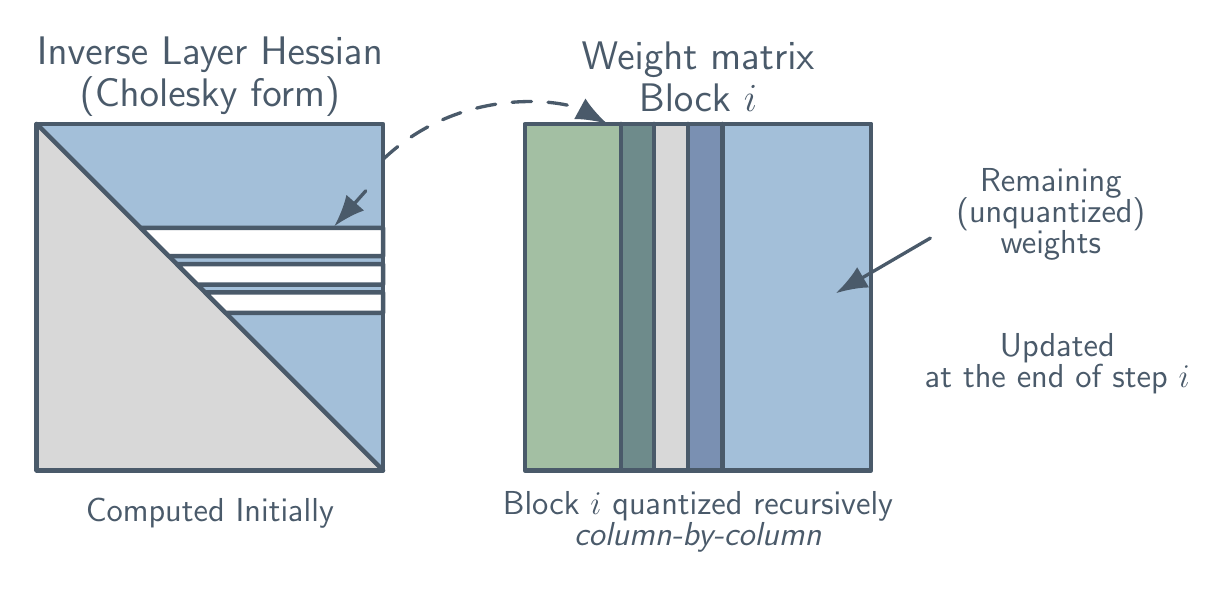
\begin{tikzpicture}[
    line join=round,
    line cap=round,
    >=Latex,
    thick,
    label/.style={font=\sffamily\Large, align=center, text=deepmutedblue},
    note/.style={font=\sffamily\large, align=center, text=deepmutedblue},
    arrow/.style={-{Latex[length=4mm,width=3mm]}, very thick, deepmutedblue},
    dashedarrow/.style={
        -{Latex[length=4mm,width=3mm]},
        very thick,
        dashed,
        dash pattern=on 7pt off 6pt,
        deepmutedblue
    }
]

% -------------------------------------------------
% Muted palette
% -------------------------------------------------
\definecolor{mistyblue}{HTML}{A3BFD9}     % Muted steel blue
\definecolor{slateblue}{HTML}{7A90B2}     % Muted slate blue
\definecolor{sagegreen}{HTML}{A3BFA3}     % Muted sage green
\definecolor{dustyteal}{HTML}{6E8B8B}     % Muted dusty teal
\definecolor{softgray}{HTML}{D8D8D8}      % Light neutral gray
\definecolor{deepmutedblue}{HTML}{4A5A6A} % Dark muted navy

% -------------------------------------------------
% Left panel
% -------------------------------------------------
\def\Lx{0}
\def\Ly{0}
\def\S{4.4}

\node[label] at (\Lx+2.2,\Ly+5.0)
{Inverse Layer Hessian\\[-1mm](Cholesky form)};

% Base square
\path[fill=mistyblue] (\Lx,\Ly) rectangle ++(\S,\S);
\path[fill=softgray]  (\Lx,\Ly) -- (\Lx,\Ly+\S) -- (\Lx+\S,\Ly) -- cycle;

\draw[ultra thick, deepmutedblue] (\Lx,\Ly) rectangle ++(\S,\S);
\draw[ultra thick, deepmutedblue] (\Lx,\Ly+\S) -- (\Lx+\S,\Ly);

% White bars connected to the diagonal
\foreach \yl/\yh in {2.72/3.08,2.36/2.62,2.00/2.26} {
    \path[fill=white]
        ({\Lx+\S-\yh},\Ly+\yh) --
        (\Lx+\S,\Ly+\yh) --
        (\Lx+\S,\Ly+\yl) --
        ({\Lx+\S-\yl},\Ly+\yl) -- cycle;

    \draw[ultra thick, deepmutedblue]
        ({\Lx+\S-\yh},\Ly+\yh) --
        (\Lx+\S,\Ly+\yh) --
        (\Lx+\S,\Ly+\yl) --
        ({\Lx+\S-\yl},\Ly+\yl) -- cycle;
}

\node[note] at (\Lx+2.2,\Ly-0.55) {Computed Initially};

% -------------------------------------------------
% Right panel
% -------------------------------------------------
\def\Rx{6.2}
\def\Ry{0}
\def\W{4.4}
\def\H{4.4}

\node[label] at (\Rx+2.2,\Ry+5.0)
{Weight matrix\\[-1mm]Block $i$};

% Columns
\path[fill=sagegreen]  (\Rx,\Ry) rectangle ++(1.22,\H);
\path[fill=dustyteal]  (\Rx+1.22,\Ry) rectangle ++(0.42,\H);
\path[fill=softgray]   (\Rx+1.64,\Ry) rectangle ++(0.43,\H);
\path[fill=slateblue]  (\Rx+2.07,\Ry) rectangle ++(0.44,\H);
\path[fill=mistyblue]  (\Rx+2.51,\Ry) rectangle ++(1.89,\H);

\draw[ultra thick, deepmutedblue] (\Rx,\Ry) rectangle ++(\W,\H);
\foreach \xx in {1.22,1.64,2.07,2.51} {
    \draw[ultra thick, deepmutedblue] (\Rx+\xx,\Ry) -- ++(0,\H);
}

\node[note] at (\Rx+2.2,\Ry-0.65)
{Block $i$ quantized recursively\\[-1mm]\textit{column-by-column}};

% -------------------------------------------------
% Arrows
% -------------------------------------------------

% Dashed curved arrow between panels
\draw[dashedarrow]
    (\Lx+\S,\Ly+3.95)
    .. controls (\Lx+\S+1.0,\Ly+4.9) and (\Rx+0.5,\Ry+4.7) ..
    (\Rx+1.05,\Ry+\H);

% Left arrow
\draw[arrow]
    (\Lx+4.18,\Ly+3.55) -- (\Lx+3.78,\Ly+3.10);

% Right annotation arrow
\draw[arrow]
    (\Rx+5.15,\Ry+2.95) -- (\Rx+3.95,\Ry+2.25);

\node[note, anchor=west] at (\Rx+5.35,\Ry+3.25)
{Remaining\\[-1mm](unquantized)\\[-1mm]weights};

\node[note, anchor=west] at (\Rx+4.95,\Ry+1.35)
{Updated\\[-1mm]at the end of step $i$};

\end{tikzpicture}
\end{document}
